
\section{Interventions on the real shortcut (A24, A26) and questions where the cue points away}

\begin{table}[tbp]
  \centering
  \footnotesize
  \setlength{\tabcolsep}{3pt}
\resizebox{\linewidth}{!}{%
  \begin{tabular}{@{}p{0.31\linewidth}lp{0.2\linewidth}p{0.36\linewidth}@{}}
    \toprule
    Attempt (Med-CMR shortcut) & Amend. & Registration & Outcome \\
    \midrule
    Test-time filler, cue preserved (L1) & A12 & pre-registered & not evaluable: the filler alone lowers accuracy (validity check failed) \\
    Option-length rewrite, attempt 1 & A6 & pre-registered & not evaluable: gate G1 failed (17.6\% of questions passed, 60\% required); no model run on the rewrites \\
    Option-length rewrite, attempt 2 & A7 & pre-registered & not evaluable: gates G1a and G1c failed (5.2\% passed); no model run on the rewrites \\
    Alarm combiner (M1) & A12 & pre-registered & falsified \\
    Saturation-aware weighting (M2) & A12 & pre-registered & falsified \\
    Product of experts, neural bias expert (M-F) & A18 & pre-registered & collapse to chance accuracy \\
    Tempered product of experts (bias temperature 3) & A20 & exploratory & falsified in 0 of 3 seeds \\
    Explicit length prior (LP) & A24 & pre-registered (E1) & criterion not met: image effect $+0.7$ to $+2.2$ points \\
    Mismatched-image uniformity (MU) & A24 & pre-registered (E1) & criterion not met: image effect $0.0$ to $+4.6$ points \\
    LP and MU together & A24 & pre-registered (E1) & criterion not met: image effect $+0.5$ to $+3.2$ points at $79$--$80\%$ accuracy \\
    \midrule
    Gold-unlikelihood under a mismatched image (UL) & A26 & criterion chosen after A24 & met in three of three seeds; success is post hoc \\
    \bottomrule
  \end{tabular}}
  \caption{\textbf{Attempts to undo the Med-CMR shortcut.} The ten rows above UL are the attempts that preceded it; UL is listed for comparison. Registration status follows the amendment records; the A6 and A7 outcomes were checked against their result files (lr\_rewrite\_attempt1 and lr\_rewrite2).}
  \label{tab:attempts}
\end{table}

\label{app:a24}

\paragraph{A24: three methods on Med-CMR.}
A24 was pre-registered after the earlier attempts failed and before its runs (the methods are called M1, M2, M3 in the amendment: LP, MU and LP+MU here).
All methods fine-tune Qwen2.5-VL-3B with the recipe of A9 (one epoch, LoRA $r=16$, learning rate $10^{-4}$, A30 GPUs), three seeds each.
\textbf{LP:} product-of-experts with an explicit bias expert, the empirical probability that the option with a given character-length rank is correct (rank 1 to 5: $0.917$, $0.056$, $0.016$, $0.007$, $0.004$, estimated on the training questions), which cannot saturate as the neural expert did.
\textbf{MU:} the standard loss plus $\mathrm{KL}(\text{uniform}\,\|\,p)$ for the same question shown with the image of another training case of the same modality and organ system, which requires comparing image and question (a blank image would only teach the model to recognise the blank image); donors exist for 9{,}175 of 9{,}277 training questions.
\textbf{LP+MU:} both.
Criterion E1, fixed in advance and applied per method with a Bonferroni-corrected level: in at least two of three seeds an image effect of at least $+5$ points on the 410 questions that the A9 reference model found text-undecided (exact McNemar $p<0.0167$) and FRESH3000 accuracy with the true image of at least $93.5\%$.
No method meets it (Table~\ref{tab:a24}); the evaluation sets had been used for the earlier attempts and no hyper-parameter was tuned on them.

\begin{table*}[t]
  \centering
  \footnotesize
  \setlength{\tabcolsep}{4pt}
  \begin{tabular}{@{}llccccccc@{}}
    \toprule
    Method & Seed & Effect, A9-LO set ($p$) & FRESH acc. & TEST711 acc. & Shortest (\%) & HI changed & Own-LO effect & All-question gap \\
    \midrule
    LP length prior & 31 & +0.73 (0.74) & 92.43 & 93.0 & 87.9 & 2 & $-0.4$ & $-0.07$ \\
     & 32 & +2.20 (0.12) & 92.33 & 93.0 & 88.2 & 1 & +2.6 & +0.37 \\
     & 33 & +1.46 (0.36) & 91.53 & 92.3 & 87.2 & 4 & +0.6 & $-0.03$ \\
    MU mismatched image & 31 & 0.00 (1.0) & 94.23 & 94.9 & 90.2 & 0 & +0.5 & +0.47 \\
     & 32 & +4.63 (0.034) & 94.70 & 94.7 & 89.9 & 0 & +0.9 & +0.80 \\
     & 33 & +0.49 (0.91) & 94.57 & 94.9 & 90.6 & 0 & +0.2 & +0.13 \\
    LP+MU both & 31 & +3.17 (0.17) & 79.93 & 81.3 & 77.1 & 155 & +30.0 & +8.33 \\
     & 32 & +1.95 (0.39) & 79.37 & 80.6 & 76.0 & 150 & +22.0 & +5.20 \\
     & 33 & +0.49 (0.90) & 79.30 & 80.7 & 76.9 & 94 & +5.9 & +0.23 \\
    \bottomrule
  \end{tabular}
  \caption{\textbf{Interventions on the real Med-CMR shortcut (A24).} Effect: true minus black image accuracy (points) on the A9 low-confidence set with exact McNemar $p$; accuracies in \%; shortest: share of shortest-option predictions on TEST711 (reference 90--92\%); HI changed: text-decisive answers (own stratum) changed by a counterfactual image; own-LO effect and all-question gap: image effect (points) on the model's own text-undecided stratum and on all 3{,}000 questions (reported, not tested). Reference model A9: FRESH accuracy 95.5\%, image effect on its own undecided set $-1.0$.}
  \label{tab:a24}
\end{table*}

Only LP+MU makes answers depend on the image at all, at a cost of about 15 points of accuracy; the all-question gap is $+8.3$ and $+5.2$ points in two seeds and $+0.2$ in the third, so we do not read this as a result.
MU has only 206--466 text-decisive questions in its own stratum (about 2{,}500 for the reference), because the penalty lowers its confidence under a black image.

\paragraph{Questions where the cue points away (exploratory).}
Of the 3{,}000 unseen questions of FRESH3000, 235 have a correct option that is \emph{not} the shortest.
On them the A9 models gain nothing from the image (Table~\ref{tab:contra}), although the length cue cannot be what decides there.
This is an exploratory analysis of existing outputs (written after A22, before the A24 results; $n=235$, differences not significant), so the safe reading is that we found no evidence (approximate 95\% intervals of the difference, from the discordant pairs: $[-4.7,+2.2]$ for Qwen-3B and $[-2.9,+2.9]$ for Qwen-7B, which exclude $+5$ points; the test is only informative for large effects) of an image benefit where the cue does not apply, which means that the cue is not shown to be the only reason why the fine-tuned models ignore the image on Med-CMR, or that these questions can mostly be answered from the text.

\begin{table}[tbp]
  \centering
  \footnotesize
  \setlength{\tabcolsep}{2.4pt}
  \begin{tabular}{@{}llccc@{}}
    \toprule
    Model & Correct option & $n$ & Acc.\ true / black & Effect ($p$) \\
    \midrule
    A9 Qwen-3B & not the shortest & 235 & 66.8 / 68.1 & $-1.3$ (0.63) \\
     & the shortest & 2{,}765 & 97.9 / 98.0 & $-0.0$ (1.0) \\
    A9 Qwen-7B & not the shortest & 235 & 72.3 / 72.3 & $+0.0$ (1.0) \\
     & the shortest & 2{,}765 & 98.0 / 97.8 & $+0.3$ (0.14) \\
    \bottomrule
  \end{tabular}
  \caption{\textbf{Image benefit by whether the cue applies (FRESH3000, A9 models).} Accuracy (\%) with the true and the black image and the difference in points with exact McNemar $p$.}
  \label{tab:contra}
\end{table}

\paragraph{A26.}
Pre-registered after A24 and before its runs; its thresholds were chosen after seeing A24 (the stated post-hoc origin).
Criterion F1: an image effect (true minus black accuracy) over all 3{,}000 FRESH questions of at least $+3$ points with exact McNemar $p<0.025$; F2: FRESH accuracy with the true image of at least $88\%$; a new method succeeds if both hold in at least two of three seeds.
Methods (Qwen-3B, A9 recipe): \textbf{UL}, the standard loss plus $-\log(1-p_{\rm gold})$ for the same question shown with the image of another case of the same modality and organ system ($\lambda=1$); \textbf{LP+UL}, UL with the length prior as bias expert; and two further seeds of LP+MU.
Table~\ref{tab:a26} gives the runs.
UL meets F1 and F2 in three of three seeds; LP+UL collapses (the main model learns to avoid the option favoured by the length prior); LP+MU meets F1 in four of five seeds and F2 in none.

\begin{table*}[t]
  \centering
  \footnotesize
  \setlength{\tabcolsep}{4pt}
\resizebox{\linewidth}{!}{%
  \begin{tabular}{@{}llccccccc@{}}
    \toprule
    Method & Seed & Effect vs black (pts) & FRESH acc. & TEST711 acc. & Shortest (\%) & True / black / random / plausible wrong (\%) & F1 & F2 \\
    \midrule
    UL & 41 & +52.4 & 91.23 & 92.5 & 86.9 & 91.2 / 38.8 / 16.2 / 79.6 & yes & yes \\
     & 42 & +68.6 & 90.27 & 91.1 & 87.1 & 90.3 / 21.6 / 13.9 / 78.8 & yes & yes \\
     & 43 & +71.0 & 89.47 & 92.5 & 88.2 & 89.5 / 18.5 / 12.7 / 77.7 & yes & yes \\
    LP+UL & 41--43 & $+0.1$, $-0.1$, 0.0 & 0.53, 0.77, 0.73 & 0.7, 0.6, 0.4 & 0.0 & collapsed & no & no \\
    LP+MU & 31 & +8.3 & 79.93 & 81.3 & 77.1 & 79.9 / 71.6 / 48.6 / 76.7 & yes & no \\
     & 32 & +5.2 & 79.37 & 80.6 & 76.0 & 79.4 / 74.2 / 56.8 / 77.8 & yes & no \\
     & 33 & +0.2 & 79.30 & 80.7 & 76.9 & 79.3 / 79.1 / 66.4 / 78.0 & no & no \\
     & 34 & +3.5 & 77.13 & 76.4 & 72.9 & 77.1 / 73.6 / 60.8 / 75.2 & yes & no \\
     & 35 & +5.0 & 77.67 & 79.6 & 75.5 & 77.7 / 72.7 / 62.0 / 75.6 & yes & no \\
    \bottomrule
  \end{tabular}}
  \caption{\textbf{A26 runs on the real Med-CMR shortcut (Qwen-3B).} Effect: true minus black image accuracy over all 3{,}000 FRESH questions (all $p<10^{-10}$ except LP+MU seed 33, $p=0.73$, and LP+UL); accuracies in \%; shortest: share of shortest-option predictions on TEST711 (reference 90--92\%). The last accuracy column gives the FRESH accuracy with the true image, a black image, a random other image and a nearest-neighbour (plausible wrong) image (exploratory).}
  \label{tab:a26}
\end{table*}

\sloppy
\paragraph{The price of image use (exploratory).}
Table~\ref{tab:price} gives, for every method tried on the real shortcut, the accuracy with the true image and the accuracy lost when the image is replaced by a plausible wrong one of the same modality (the figure on the price of image use in the main paper).
The black-image effect of UL ($+52$ to $+71$ points) is inflated by the penalty itself: the penalty lowers the probability of the correct option under images of other cases, so a black or unrelated image is treated alike, and with a random other image the accuracy of UL is $12.7$--$16.2\%$, below chance.
The loss against a plausible wrong image is the more conservative measure of dependence on the specific image; it does not separate dependence on image content from detecting a mismatch of modality or organ.

\begin{table}[tbp]
  \centering
  \footnotesize
  \setlength{\tabcolsep}{2.4pt}
\resizebox{\linewidth}{!}{%
  \begin{tabular}{@{}lccc@{}}
    \toprule
    Method (seeds) & Acc.\ true image & Loss, plausible wrong image & Loss, random image \\
    \midrule
    Reference (A9) & 95.5 & 0.0 & $-0.1$ \\
    Tempered expert (3) & 95.0--95.7 & 0.2--0.3 & 0.0--0.4 \\
    LP (3) & 91.5--92.4 & 0.0--0.4 & 0.0--0.3 \\
    MU (3) & 94.2--94.7 & 1.1--1.3 & 22.7--27.5 \\
    LP+MU (5) & 77.1--79.9 & 1.3--3.3 & 12.9--31.3 \\
    UL (3) & 89.5--91.2 & 11.5--11.8 & 75.0--76.8 \\
    \bottomrule
  \end{tabular}}
  \caption{\textbf{Price of image use on the real shortcut} (FRESH3000, accuracy in \%, losses in points relative to the true image).}
  \label{tab:price}
\end{table}

\paragraph{Blur test of the UL models (A27).}
Pre-registered after A26 and run on the saved adapters (evaluation only): FRESH3000 accuracy with the true image blurred (Gaussian radius 32, 16, 8, 4, 2 px) and intact (UL seed 41: 43.8, 61.7, 81.3, 89.0, 90.6 and 91.2\% at blur 32, 16, 8, 4, 2 and intact, against 38.8\% with a black image; the other seeds and the control models are in the released result record).
Rule C (rise of at least 10 points from blur 32 to the intact image, no level-to-level fall larger than 1 point) holds in three of three UL seeds.
By the reading rule fixed in advance, R8 $\ge0.8$ in two of three seeds (R8 is the share of the gap between the black and the intact image that is recovered at blur 8), so the dependence rests mostly on coarse image identity (modality, organ, global appearance), consistent with detection of a mismatch, although the accuracy still improves with sharpness; LP+MU (rise 0.0 and 1.2 points) and the reference are flat.


\section{Where the lock-out lies, relative to the benefit without a cue}
\label{app:rel}

Because the benefit at $d=0.25$ differs (about $+13.5$ points on PMC-VQA, $+34$ on A-OKVQA), Table~\ref{tab:rel} gives the benefit as a share of its value at $d=0.25$ and the strength at which this share falls to 20\% and 10\%, interpolated linearly in the logit of $d$ between the tested strengths (exploratory; the grids are coarse, so only the bracket is certain).
The ordering of the benchmarks does not depend on the absolute $+2$ threshold of the veto boundary: PMC-VQA crosses 20\% between $d=0.70$ and $0.85$ (Qwen-3B; the other models only between $0.70$ and $0.92$), A-OKVQA between $0.92$ and $0.97$ (Qwen-3B) and between $0.92$ and $0.99$ (Qwen-7B and InternVL3-2B, whose $d=0.99$ run is a single seed).
InternVL3-2B on A-OKVQA still has 31\% of its benefit at $d=0.92$.

\begin{table}[tbp]
  \centering
  \footnotesize
  \setlength{\tabcolsep}{2.4pt}
  \resizebox{\linewidth}{!}{%
\begin{tabular}{@{}llcccc@{}}
    \toprule
    Benchmark & Model (seeds) & $g$(0.25) & $d$ at 20\% & $d$ at 10\% & share at 0.92 \\
    \midrule
    PMC-VQA & Qwen-3B (3) & 13.5 & 0.74 & 0.81 & 0.7\% \\
     & Qwen-7B (2) & 15.4 & 0.79 & 0.87 & 1.1\% \\
     & InternVL3-2B (2) & 13.4 & 0.71 & 0.85 & 0.7\% \\
    A-OKVQA & Qwen-3B (2--3) & 33.6 & 0.94 & 0.97 & 24.2\% \\
     & Qwen-7B (2) & 35.1 & 0.93 & 0.97 & 20.8\% \\
     & InternVL3-2B (1--2) & 38.3 & 0.97 & 0.98 & 31.3\% \\
    \bottomrule
  \end{tabular}}
  \sloppy \caption{\textbf{Benefit relative to the benefit without a cue.} $g$(0.25): mean image benefit (points) at $d=0.25$; $d$ at 20\% and 10\%: interpolated strength at which the benefit falls to that share of $g$(0.25) (--: not reached within the tested strengths); share at 0.92: benefit at $d=0.92$ as a share of $g$(0.25).}
  \label{tab:rel}
\end{table}

\section{Seeds behind each claim, and the benchmark audit}
\label{app:seeds}

\begin{table}[tbp]
  \centering
  \footnotesize
  \setlength{\tabcolsep}{2.4pt}
  \begin{tabular}{@{}p{0.34\columnwidth}p{0.26\columnwidth}p{0.3\columnwidth}@{}}
    \toprule
    Claim & Benchmark & Seeds per model \\
    \midrule
    Dose-response, length & PMC-VQA & Qwen-3B 3; Qwen-7B 2; InternVL3-2B 2 \\
     & A-OKVQA & Qwen-3B 3; Qwen-7B 2; InternVL3-2B 2 \\
    Lock-out ($V^\ast=$ none) & PMC-VQA, $d\ge0.85$ & Qwen-3B 3; $d=0.92$: Qwen-7B 2, InternVL3-2B 2 \\
     & A-OKVQA, $d=0.99$ & Qwen-3B 3; Qwen-7B 2; InternVL3-2B 1 (not locked: $+1.7$) \\
    Second shortcut (position) & PMC-VQA; A-OKVQA & Qwen-3B 1 each \\
    Held-out prediction & PMC-VQA & Qwen-7B 2; InternVL3-2B 2 \\
    Real-shortcut methods & Med-CMR & Qwen-3B 3 each (A18, A20, LP, MU, LP+MU) \\
    \bottomrule
  \end{tabular}
  \caption{\textbf{Number of seeds behind each claim.} Seeds differ in the training order and the LoRA initialisation; the planted cue assignment is fixed by question.}
  \label{tab:seeds-sup}
\end{table}

\paragraph{Option-length and position audit of seven benchmarks (A28).}
\label{sec:supp-audit}
Exploratory, text only, run before its amendment was written and frozen with its script and output (no model, no image).
The \emph{shortest-option rule} picks the shortest option (ties split); the table gives its accuracy against chance, and the most frequent position of the correct option.
\begin{center}
\footnotesize
\setlength{\tabcolsep}{4pt}
\resizebox{\linewidth}{!}{%
\begin{tabular}{@{}lrrrl@{}}
\toprule
Benchmark & $n$ & rule & chance & correct option most often at\\
\midrule
Med-CMR (train MCQ) & 14{,}398 & \textbf{91.9} & 20.0 & A (20.7\%)\\
PMC-VQA train & 176{,}934 & 30.3 & 25.0 & B (30.6\%)\\
PMC-VQA clean test & 2{,}000 & 24.4 & 25.0 & B (31.9\%)\\
OmniMedVQA (open access) & 88{,}996 & 32.7 & 26.9 & B (26.9\%)\\
A-OKVQA (val) & 1{,}145 & 23.6 & 25.0 & C (25.8\%)\\
MedXpertQA-MM~\cite{zuo2025medxpertqa} (test) & 2{,}000 & 18.4 & 20.0 & E (21.2\%)\\
MMMU~\cite{yue2024mmmu} health (val, MCQ) & 145 & 29.1 & 26.5 & A (31.0\%)\\
\bottomrule
\end{tabular}}
\end{center}
Only Med-CMR carries a severe length cue (excess over chance $+71.9$ points; all others between $-1.6$ and $+5.8$).
OmniMedVQA mixes two-, three- and four-option items, so its chance level is 26.9\% and its excess is $+5.8$.
PMC-VQA has a weak position skew (correct option B in about 31\% of questions) and a training-set length rule slightly above chance ($+5.3$) that is absent in its clean test set.
Limits: two cue types (character length, position); MMMU is small; GMAI-MMBench~\cite{chen2024gmai} is gated and was not examined; we make no claim about image use in the other sets from this audit.

\paragraph{Option-text audit of Med-CMR (A31).}
Text only (neither image nor, except for one overlap feature, question), exploratory in the sense that its features were fixed before the run but not tuned.
Option-level logistic regression, trained on the 13{,}687 training MCQs outside the held-out list and tested on the 711 held-out MCQs, 56 of which are \emph{cue-contradicting} (correct option not the shortest; chance among the other four options 25\%).
\begin{center}
\footnotesize
\setlength{\tabcolsep}{3pt}
\resizebox{\linewidth}{!}{%
\begin{tabular}{@{}lcc@{}}
\toprule
Model (features; training questions) & all 711 & 56 cue-contradicting\\
\midrule
M0 shortest-option rule & 91.1 & 0.0\\
M1 length features; all & 91.0 & 3.6 [0.0, 8.9]\\
M2 word and bigram TF-IDF; all & 90.0 & 64.3 [51.8, 76.8]\\
M3 TF-IDF; cue-contradicting only & 71.6 & 51.8 [39.3, 64.3]\\
M4 non-length style features; all & 75.0 & 23.2 [12.5, 33.9]\\
M5 style features; cue-contradicting only & 58.2 & 35.7 [23.2, 50.0]\\
M6 TF-IDF + style; cue-contradicting only & 73.0 & 55.4 [42.9, 67.9]\\
\bottomrule
\end{tabular}}
\end{center}
Both pre-registered rules hold (M3 on cue-contradicting questions at least $35\%$ with lower bound at least $28\%$; M4 on all questions at least $60\%$).
The wording of the correct option therefore identifies it beyond character length: M2 and M3 pick the correct option in $52$--$64\%$ of the questions in which it is not the shortest, picking the shortest in only $11$--$20\%$.
Limits: 56 test questions and wide intervals; n-grams and style features such as the overlap with the other options are not independent of length; 47 test MCQs have a near-duplicate partner in the pool; we do not test what a language model reads, nor which wording carries the signal.

\paragraph{A stratifier that uses neither the model nor an image (A32).}
Text confidence: the top probability of the within-question softmax over the five option scores of a word and bigram TF-IDF classifier (out-of-fold, folds grouped by near-duplicate component); FRESH3000 in terciles.
Qwen-3B (Qwen-7B): top tercile, accuracy with the true / black image $100.0/100.0$ ($99.8/100.0$), image effect $0.0$ ($-0.2$), answers changed relative to the black / random / plausible-wrong image $0.0/0.0/0.0\%$ ($0.2/0.0/0.1\%$); middle tercile effect $+0.1$ ($0.0$); bottom tercile (least predictable) $87.8/88.3$ ($89.1/88.2$), effect $-0.5$ ($+0.9$), $p=0.46$ ($0.12$), changed $3.9/3.6/2.3\%$ ($3.1/3.0/1.7\%$).
Both pre-registered rules hold (top tercile at most 2.0\% changed; Spearman correlation of the text confidence with the model's black-image margin $0.68$ and $0.71\ge0.4$).
Even the least text-predictable third is answered 88--89\% correctly with a black image, so the fine-tuned models have more text-side ability than this classifier captures.

\paragraph{The wording signal at scale (A33).}
All 14{,}398 MCQs, 1{,}023 of them cue-contradicting (1{,}020 near-duplicate components); out-of-fold accuracy on those, with 95\% intervals resampled by component (chance 25\%).
TF-IDF trained on all questions $55.0$ [51.8, 58.2], on cue-contradicting questions only $47.9$ [44.9, 51.2]; single style groups: word overlap with the other options $43.7$ [40.8, 46.9], with the question $28.3$ [25.5, 31.3], commas per word $23.7$ [21.2, 26.1], hedging, negation at the start and digits $19.9$--$21.0$; all style groups together $46.8$ [43.9, 50.1]; the shortest option is picked in $14$--$27\%$ of these questions by these classifiers.
Strongest terms for correct options: right, structures, across, localized to, uncommon, established, indicates an, rounded, widespread, heterogeneous; for wrong options: without, suggesting, only, but, no, focal, predominantly, not, minimal, preserved, limited, rather than, confined.
Both pre-registered rules hold; the terms are associations, not causes.

\paragraph{Average measures against the stratified view (A34).}
\begin{center}
\footnotesize
\setlength{\tabcolsep}{3pt}
\resizebox{\linewidth}{!}{%
\begin{tabular}{@{}lrrrrr@{}}
\toprule
System (one seed) & drop & VIG & changed & decisive / changed & undecided effect\\
\midrule
Med-CMR Qwen-3B & $-0.1$ & $0.00$ & 1.3\% & 76\% / 0.0\% & $-1.0$ (410)\\
Med-CMR Qwen-7B & $+0.2$ & $0.00$ & 1.1\% & 79\% / 0.0\% & $+1.8$ (386)\\
PMC-VQA Qwen-3B & $+12.9$ & $0.16$ & 41.7\% & 0\% / -- & $+12.9$ (3000)\\
PMC-VQA Qwen-7B & $+12.6$ & $0.17$ & 41.3\% & 0\% / -- & $+12.6$ (3000)\\
PMC-VQA InternVL3-2B & $+9.8$ & $0.14$ & 40.0\% & 0\% / -- & $+9.8$ (3000)\\
OmniMedVQA Qwen-3B & $+6.3$ & $0.16$ & 7.1\% & 64\% / 0.1\% & $+27.3$ (652)\\
OmniMedVQA Qwen-7B & $+6.9$ & $0.20$ & 7.4\% & 65\% / 0.7\% & $+25.3$ (687)\\
OmniMedVQA InternVL3-2B & $+15.9$ & $0.58$ & 16.8\% & 49\% / 1.8\% & $+40.0$ (927)\\
\bottomrule
\end{tabular}}
\end{center}
drop: accuracy with the true minus the black image (points); VIG: mean gain in the gold log-probability from the image (nats); changed: share of answers changed by the black image; decisive: black-image margin of at least 0.99 and the share of their answers changed; undecided: black-image margin below 0.90, its image effect in points and size.
Spearman correlation across the eight systems: drop against VIG $0.69$, against the share changed $0.83$ (rule: $\ge0.9$ for both; failed).
The text-decisive stratum defined by the 15th percentile of unlabeled margins is not comparable across benchmarks (the threshold is $0.04$ on PMC-VQA), hence the 0.99 column.
Limits: eight systems, one seed each; the released adapter is not included.

\paragraph{Centre versus border occlusion (A35).}
Evaluation only, saved Qwen-3B adapters, planted options of their training; half of the image area set to black, either the central rectangle or the complementary frame.
\begin{center}
\footnotesize
\setlength{\tabcolsep}{3pt}
\resizebox{\linewidth}{!}{%
\begin{tabular}{@{}lccccc@{}}
\toprule
Adapter (seed) & true & black & centre occluded & border occluded & centre $-$ border\\
\midrule
PMC-VQA $d=0.25$ (1011) & 50.98 & 37.22 & 45.87 & 46.97 & $-1.10$\\
PMC-VQA $d=0.25$ (1012) & 50.98 & 38.12 & 46.57 & 47.77 & $-1.20$\\
PMC-VQA $d=0.25$ (1013) & 50.58 & 36.77 & 45.82 & 46.42 & $-0.60$\\
PMC-VQA $d=0.70$ (1011) & 72.09 & 68.53 & 70.74 & 71.34 & $-0.60$\\
PMC-VQA $d=0.70$ (1012) & 71.94 & 68.68 & 70.29 & 71.24 & $-0.95$\\
PMC-VQA $d=0.70$ (1013) & 72.39 & 69.13 & 70.84 & 71.74 & $-0.90$\\
A-OKVQA $d=0.25$ (1021) & 82.53 & 48.65 & 69.00 & 78.86 & $-9.86$\\
A-OKVQA $d=0.25$ (1022) & 83.06 & 49.78 & 68.82 & 79.74 & $-10.92$\\
\bottomrule
\end{tabular}}
\end{center}
Accuracy (\%) on E1 (1{,}999 and 1{,}145 questions).
Rule O1 (PMC-VQA, $d=0.25$: centre lower than border by at least 2.0 points in two of three seeds) fails; rule O2 (A-OKVQA, both seeds) holds.
Under centre occlusion the adapters lose 34--37\% (PMC-VQA, $d=0.25$) and 40--43\% (A-OKVQA) of their true-minus-black benefit, under border occlusion 25--30\% and 10--11\%.
Limits: medical and natural images are usually centred, so a central preference may reflect composition; two region definitions; one model size; not an attention analysis.

\paragraph{UL on Qwen2.5-VL-7B (A30).}
Same method and recipe as A26 (penalty weight 1, one epoch, gradient checkpointing), seeds 20261051 and 20261052; FRESH3000.
\begin{center}
\footnotesize
\setlength{\tabcolsep}{3pt}
\resizebox{\linewidth}{!}{%
\begin{tabular}{@{}lccccccc@{}}
\toprule
Seed & true & black & random other & plausible wrong & blur 32 / 16 / 8 & blur 4 / 2 & intact\\
\midrule
20261051 & 90.50 & 82.47 & 9.30 & 73.03 & 12.9 / 40.2 / 77.2 & 87.5 / 90.2 & 90.50\\
20261052 & 89.63 & 77.60 & 8.70 & 71.83 & 15.7 / 45.0 / 79.0 & 86.9 / 88.6 & 89.63\\
\bottomrule
\end{tabular}}
\end{center}
Image effect $+8.03$ and $+12.03$ points ($p=4\times10^{-26}$ and $10^{-44}$); true minus plausible wrong image $+17.5$ and $+17.8$ points; TEST711 accuracy 90.4 and 89.7\%.
All three pre-registered rules hold in both seeds (image effect $\ge+3.0$ with accuracy $\ge88\%$; true minus plausible wrong $\ge+5.0$; rule C of A27 on the blur ladder).
$R_8=-0.65$ and $+0.12$ (below 0.8), but this index is hard to read here because blur 32 and 16 give accuracy far below the black image, i.e. heavily blurred images mislead the model more than no image.
The black-image effect is much smaller than at 3B ($+8$ and $+12$ against $+52$ to $+71$ points) because the 7B models keep 78--82\% accuracy with a black image.
Limits: two seeds, one penalty setting.

\paragraph{Counter-cue accuracy and the blind ceiling (A36).}
\emph{Counter-cue questions} are those whose correct option is not the (tied) shortest: 206 of the 3{,}000 FRESH questions (235 if ties are counted), 1{,}023 of the 14{,}398 training MCQs (ids released).
\begin{center}
\footnotesize
\setlength{\tabcolsep}{3pt}
\resizebox{\linewidth}{!}{%
\begin{tabular}{@{}lcccc@{}}
\toprule
System (FRESH3000) & counter-cue, true image & counter-cue, black & cue-following, true & gap\\
\midrule
A9 Qwen-3B & 68.0 [61.6, 74.3] & 68.9 & 97.5 & 29.6\\
A9 Qwen-7B & 73.3 [66.5, 79.1] & 73.3 & 97.7 & 24.4\\
UL Qwen-3B (3 seeds) & 57.8--62.1 & 15.5--29.6 & 91.8--93.4 & 31.2--34.0\\
UL Qwen-7B (2 seeds) & 59.2--63.1 & 52.4--53.9 & 91.9--92.5 & 29.4--32.7\\
LP+MU Qwen-3B (5 seeds) & 61.2--62.6 & 55.8--60.7 & 78.3--81.3 & 16.7--20.2\\
\bottomrule
\end{tabular}}
\end{center}
The pre-registered expectation that the two reference models lose at least 30 points failed (29.6 and 24.4), so the gap is smaller than the error analysis suggested; for the reference models a black image changes the counter-cue accuracy by about a point.
\begin{center}
\footnotesize
\setlength{\tabcolsep}{3pt}
\resizebox{\linewidth}{!}{%
\begin{tabular}{@{}lcccccc@{}}
\toprule
Benchmark & $n$ test & chance & blind ceiling & Qwen-3B true / black & visual headroom\\
\midrule
Med-CMR & 711 & 20.0 & 93.7 [91.7, 95.4] & 95.5 / 95.6 & $-0.1$\\
OmniMedVQA & 2{,}000 & 27.0 & 94.1 [92.9, 95.1] & 98.9 / 93.2 & $+4.9$\\
PMC-VQA & 2{,}000 & 25.0 & 29.5 [27.6, 31.5] & 51.8 / 38.1 & $+13.7$\\
A-OKVQA & 1{,}145 & 25.0 & 40.1 [37.4, 43.1] & 82.8 / 49.6 & $+33.2$\\
MedXpertQA-MM & 2{,}000 & 20.0 & 22.9 [21.1, 24.7] & -- & --\\
MMMU health & 145 & 26.5 & 23.5 [17.2, 30.3] & -- & --\\
\bottomrule
\end{tabular}}
\end{center}
Blind ceiling: accuracy of an option-level classifier (word and bigram TF-IDF of the option and four within-question length features; no question, no image), trained on the benchmark's own training questions (up to 30{,}000) or, for the last two, cross-validated within the test set; visual headroom: true-image accuracy of the fine-tuned Qwen-3B minus the larger of the blind ceiling and its black-image accuracy.
Both pre-registered rules hold (ceiling at least 85\% on Med-CMR and at most 45\% on PMC-VQA and A-OKVQA; Med-CMR has the smallest headroom).
OmniMedVQA has no length cue (A28) but a blind ceiling of 94.1\%: the answer priors of its source datasets saturate it as well, which the length audit alone misses.
Limits: the classifier does not see the question, so for PMC-VQA and A-OKVQA the ceiling is a lower bound of what text can reach; one model per benchmark; the counter-cue split is defined by length only.

\paragraph{The faithfulness gate of the challenge (A37).}
Released adapter, container code and decoding unchanged, on the 175 open-ended cases of the 886-case held-out slice; judge: Qwen2.5-VL-7B-Instruct with the scoring-suite VA rubric (VA\_answer and RVF\_trace on 0--4, VA\_final by the challenge's gate), greedy decoding, shown the true image of the case unless stated.
\begin{center}
\footnotesize
\setlength{\tabcolsep}{3pt}
\resizebox{\linewidth}{!}{%
\begin{tabular}{@{}lccccc@{}}
\toprule
Model input (judge image) & VA\_answer & RVF\_trace & VA\_final & traces saying black/blank & trace length\\
\midrule
true image (true) & 3.07 & 3.08 & 3.07 & 16.0\% & 1{,}431\\
black image (true) & 0.25 & 0.30 & 0.25 & 89.7\% & 812\\
other case's image, same modality (true) & 2.19 & 2.45 & 2.19 & 19.4\% & 1{,}423\\
true image (black) & 3.01 & 3.03 & 3.01 & -- & --\\
\bottomrule
\end{tabular}}
\end{center}
Pre-registered rules: RVF\_trace true minus black model $2.78$ [2.63, 2.90] (rule $\ge1.0$: holds); VA\_final $2.82$ [2.69, 2.93] ($\ge0.5$: holds); RVF\_trace true minus wrong-image model $0.63$ [0.46, 0.81] ($\ge1.0$: fails); RVF\_trace with the true minus a black image at the judge $0.05$ [0.02, 0.08] ($\ge0.5$: fails).
For this 7B judge the score is therefore sensitive to the trace's statement that the image is missing and insensitive both to a wrong image and to the image the judge is shown; the next paragraph repeats the tests at three judge sizes.
Limits: a reproduction judge of a different prompt and possibly size, one released system, 175 cases, no GT scoring; the first judge job failed at an import and was rerun unchanged otherwise.

\paragraph{Three judge sizes and judge-side counterfactuals (A38).}
Same outputs of the released adapter and rubric, judges Qwen2.5-VL-3B, -7B and -32B-Instruct; mean RVF\_trace (0--4) for seven conditions.
\begin{center}
\footnotesize
\setlength{\tabcolsep}{3pt}
\resizebox{\linewidth}{!}{%
\begin{tabular}{@{}lccc@{}}
\toprule
Condition & 3B & 7B & 32B\\
\midrule
C1 own trace, true image & 3.94 & 3.08 & 3.40\\
C2 own trace, black image at the judge & 3.94 & 3.03 & 3.54\\
C3 own trace, image of another case (same modality) & 3.88 & 2.81 & 2.36\\
C4 own trace, no image at the judge & 3.83 & 3.07 & 3.39\\
C5 trace and answer of another case, this case's image & 3.45 & 2.21 & 1.95\\
C6 black-image model's trace, true image & 0.41 & 0.30 & 0.32\\
C7 wrong-image model's trace, true image & 3.55 & 2.45 & 2.35\\
\bottomrule
\end{tabular}}
\end{center}
Pre-registered rules (C1 minus the condition, lower 95\% bound in brackets): K1, other case's image $\ge0.5$: $+0.06$ [0.02], $+0.27$ [0.17], $+1.04$ [0.83] (holds at 32B only); K2, another case's trace $\ge1.0$: $+0.50$ [0.36], $+0.87$ [0.69], $+1.45$ [1.21] (32B only); K3, black-image model $\ge1.0$: $+3.53$, $+2.78$, $+3.08$ (all hold).
Observed: none of the judges penalises a missing image (C2, C4); the 32B judge detects contradiction with the image but does not require visual evidence; of the 175 black-image traces, 18 do not state that the image is black or blank, and their mean score under the true image is $3.33$, $2.22$ and $2.22$ (3B, 7B, 32B), against $0.08$--$0.10$ for the others (exploratory, regex-defined).
Limits: the organisers' judge size, prompt and decoding are unknown; one system and 175 cases; same-modality swaps can give traces that are plausible for the image.

\paragraph{The released system on counter-cue and blind-fail questions (A39).}
On the 711 held-out MCQs, 56 are counter-cue and 45 are \emph{blind-fail} (an option-only classifier trained outside the held-out cases picks a wrong option; 38 questions are both).
\begin{center}
\footnotesize
\setlength{\tabcolsep}{3pt}
\resizebox{\linewidth}{!}{%
\begin{tabular}{@{}lcccc@{}}
\toprule
System & all 711 & counter-cue (56) & cue-following (655) & blind-fail (45)\\
\midrule
Released adapter (Qwen3.5-9B) & 96.1 & 83.9 [73.2, 92.9] & 97.1 & 82.2 [68.9, 93.3]\\
A9 Qwen-3B & 95.4 & 66.1 [53.6, 78.6] & 97.9 & 66.7 [53.3, 80.0]\\
A9 Qwen-7B & 95.4 & 67.9 [55.4, 80.4] & 97.7 & 66.7 [53.3, 80.0]\\
UL Qwen-3B (3 seeds) & 91.1--92.6 & 62.5--71.4 & 93.6--95.1 & 62.2--75.6\\
UL Qwen-7B (2 seeds) & 89.7--90.4 & 60.7 & 92.2--93.0 & 57.8--64.4\\
\bottomrule
\end{tabular}}
\end{center}
The pre-registered expectation that the released system falls to at most 80\% on counter-cue questions (with a gap of at least 15 points) failed (83.9\%, gap 13.2 points): it loses less than our systems, but its overall accuracy still overstates its accuracy where length misleads by about 12 points (our reference models by 27--29).
Limits: 56 and 45 questions, so wide intervals; one released system; the blind-fail definition depends on one classifier.

\paragraph{Zero-shot Qwen2.5-VL-7B on six benchmarks (A40, 7B run).}
No fine-tuning; letter log-probability readout; arms: true image(s), black image(s), and no image with the note that the image could not be loaded (told).
\begin{center}
\footnotesize
\setlength{\tabcolsep}{3pt}
\resizebox{\linewidth}{!}{%
\begin{tabular}{@{}lccccc@{}}
\toprule
Benchmark ($n$; chance) & true & black & told & blind ceiling & black $-$ chance\\
\midrule
Med-CMR (711; 20.0) & 27.6 & 27.7 & 29.1 & 93.7 & $+7.7$\\
PMC-VQA (1{,}999; 25.0) & 52.5 & 36.1 & 32.5 & 29.5 & $+11.1$\\
OmniMedVQA (2{,}000; 25.0) & 75.4 & 57.2 & 55.9 & 94.1 & $+32.2$\\
A-OKVQA (1{,}145; 25.0) & 86.0 & 46.2 & 49.3 & 40.1 & $+21.2$\\
MedXpertQA-MM~\cite{zuo2025medxpertqa} (2{,}000; 20.0) & 23.0 & 23.5 & 22.8 & 22.9 & $+3.5$\\
MMMU~\cite{yue2024mmmu} health (145; 26.5) & 51.0 & 45.5 & 46.2 & 23.5 & $+19.0$\\
\bottomrule
\end{tabular}}
\end{center}
Rule Z2 (blind ceiling minus the 7B black-image accuracy at least 30 points on Med-CMR and OmniMedVQA) holds ($66.0$ and $36.9$).
The note that the image is unavailable lowers accuracy relative to the black image on PMC-VQA, OmniMedVQA and MedXpertQA-MM and raises it on the other three (rule Z3 concerns the 32B model and rule Z1, the knowledge route on PMC-VQA, MedXpertQA-MM and MMMU health, is likewise a 32B rule; the 32B run was not performed, so Z1 and Z3 are not evaluable).
Limits: letter readout, not free generation; one model family; MMMU uses at most three images.

\paragraph{Protocol figure and the teaser example.}
\begin{figure}[h]
  \centering
  \includegraphics[width=0.95\columnwidth]{fig/f0_protocol.pdf}
  \caption{\textbf{Protocol.} Each question is run with the true image and counterfactual images (black, random, plausible wrong, and a ladder of degraded images); the model's confidence with the black image, $m_b$, defines the text-saturation stratum (threshold fixed on unlabeled data), and answers are compared across arms within each stratum.}
  \label{fig:protocol-supp}
\end{figure}
The teaser item in the main text is illustrative: its question and options are invented, it reproduces no benchmark item, and it shows no image. The numbers it summarises are the measured aggregates reported in the main text and in the tables of Supp.~M and Supp.~Z; the figure was laid out with code and its text was written for this purpose.

\paragraph{The price of image use (figure).}
\begin{figure}[h]
  \centering
  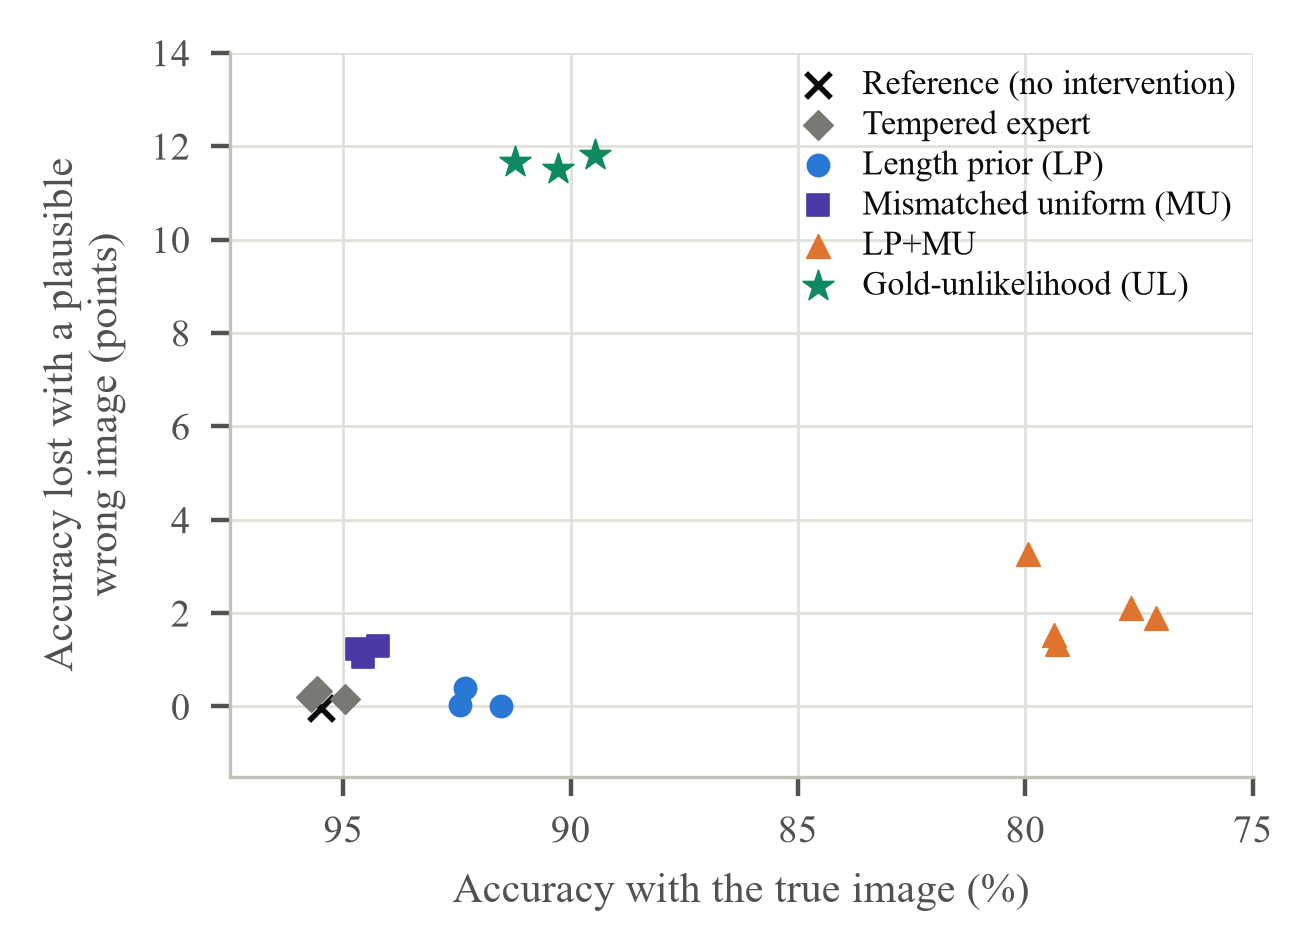
\includegraphics[width=\columnwidth]{fig/f11_price.png}
  \caption{\textbf{The price of image use on the real shortcut} (Qwen-3B, Med-CMR, 3{,}000 unseen questions, one point per run). Accuracy with the true image against the accuracy lost when the image is replaced by a plausible wrong one of the same modality; up and to the left is better.}
  \label{fig:price-supp}
\end{figure}

\paragraph{The same systems and recipe on three conditions (figure).}
\begin{figure}[h]
  \centering
  \includegraphics[width=\columnwidth]{fig/f5_two_benchmarks.pdf}
  \caption{\textbf{The same three systems and recipe on three conditions.} Orange: Med-CMR (3{,}000 unseen questions); blue: PMC-VQA (clean test, 1{,}999); violet: PMC-VQA with a length cue planted at 92\% (Sec.~5). (a)~Distribution of the black-image margin (solid, dashed, dotted: Qwen 3B, Qwen 7B, InternVL 2B). (b)~Share of predictions equal to the shortest option. (c)~Image benefit over all questions. (d)~Image benefit when the true image is blurred (radius 24 and 8\,px) or intact; mean and range over the three families.}
  \label{fig:two-supp}
\end{figure}

\paragraph{A natural dose-response, without planting anything (A42).}
Image benefit (true minus black image accuracy, points) by quintile of the text predictability of the question (option-only classifier trained on the benchmark's own training split; quintile 1 least predictable), pooled over the models of the benchmark.
\begin{center}
\footnotesize
\setlength{\tabcolsep}{3pt}
\resizebox{\linewidth}{!}{%
\begin{tabular}{@{}lcccccc@{}}
\toprule
Benchmark (questions; models) & Q1 & Q2 & Q3 & Q4 & Q5 & Spearman\\
\midrule
Med-CMR (3{,}000; 2) & $+0.3$ & 0.0 & 0.0 & 0.0 & 0.0 & $-0.71$\\
PMC-VQA (4{,}999; 3) & $+10.8$ & $+10.2$ & $+21.6$ & $+12.4$ & $+9.6$ & $-0.20$\\
OmniMedVQA (5{,}000; 3) & $+13.7$ & $+10.8$ & $+8.7$ & $+4.4$ & $+10.7$ & $-0.70$\\
A-OKVQA (1{,}145; 6) & $+35.2$ & $+33.3$ & $+40.0$ & $+34.9$ & $+34.1$ & $-0.20$\\
\bottomrule
\end{tabular}}
\end{center}
Both pre-registered rules fail (Spearman at most $-0.8$ and Q1 minus Q5 at least 5 points, each in three of four benchmarks): the largest Q1 minus Q5 difference is $+2.9$ (OmniMedVQA).
Where the blind ceiling is low the classifier's mean top probability varies only from $0.30$ to $0.51$ (PMC-VQA) and $0.30$ to $0.59$ (A-OKVQA; chance $0.25$); on Med-CMR it is $0.98$ already in the second quintile.
Limits: correlational; predictability is confounded with question type and difficulty and captures only artifacts learnable from the benchmark's training split.

\paragraph{Three things that headroom must not be confused with.}
\begin{center}
\footnotesize
\setlength{\tabcolsep}{3pt}
\resizebox{\linewidth}{!}{%
\begin{tabular}{@{}p{0.22\linewidth}p{0.36\linewidth}p{0.42\linewidth}@{}}
\toprule
Level & Tests in this paper & Status\\
\midrule
Visual information is available & every arm with the true image & given by design\\
Predictions depend on the image & black, random and plausible-wrong images; headroom; veto boundary; dose-response & tested throughout\\
The model reasons about the relevant visual content & drop under a plausible wrong image (UL: $11.6$ at 3B, $17.5$ at 7B); blur ladder (coarse identity at 3B); centre-versus-border occlusion (A-OKVQA only); judge checks (32B only) & partial; no region-level reasoning test\\
\bottomrule
\end{tabular}}
\end{center}

\paragraph{A frozen evidence-competition hypothesis for the lock-out strength (A43).}
$V$: mean over questions of $\log p(\text{gold}\mid\text{true image})-\log p(\text{gold}\mid\text{black image})$ of the cue-free ($d=0.25$) model; $S(d)=\log\frac{3d}{1-d}$ (zero at $d=0.25$); hypothesis: lock-out where $S(d^\ast)=\lambda V$, one constant $\lambda=11.1$ set on Qwen-3B/PMC-VQA.
\begin{center}
\footnotesize
\setlength{\tabcolsep}{3pt}
\resizebox{\linewidth}{!}{%
\begin{tabular}{@{}lcccc@{}}
\toprule
Condition & $V$ (nats) & predicted $S$ ($d^\ast$) & observed bracket in $d$ ($S$) & inside\\
\midrule
PMC-VQA Qwen-3B (calibration) & 0.215 & 2.39 (0.78) & 0.70--0.85 (1.95--2.83) & yes\\
PMC-VQA Qwen-7B & 0.236 & 2.62 (0.82) & 0.70--0.92 (1.95--3.54) & yes\\
PMC-VQA InternVL3-2B & 0.205 & 2.28 (0.76) & 0.70--0.92 (1.95--3.54) & yes\\
A-OKVQA Qwen-3B & 0.765 & 8.50 (0.9994) & 0.97--0.99 (4.58--5.69) & no\\
A-OKVQA Qwen-7B & 0.799 & 8.87 (0.9996) & 0.92--0.99 (3.54--5.69) & no\\
A-OKVQA InternVL3-2B & 0.987 & 10.96 (0.9999) & not locked at 0.99 & yes\\
OmniMedVQA Qwen-3B & 0.172 & 1.91 (0.69) & not locked at 0.85 & no\\
\bottomrule
\end{tabular}}
\end{center}
Inside means within 0.5 nats of the observed bracket. Rule P1 (A-OKVQA Qwen-3B) fails; P2 (three of four other conditions) holds; P3 (OmniMedVQA, prospective) fails because the prediction is already contradicted by the existing runs, so the announced runs at $d=0.92$, 0.97 and 0.99 were not performed.
P1 and P2 are retrospective (the brackets were known; only $V$ and the hypothesis were new).
The visual gain is 3.6 times larger on A-OKVQA than on PMC-VQA while the shortcut evidence at lock-out is only about 2.1 times larger, so the relation is sublinear; the hypothesis was not modified.

\paragraph{Zero-shot Qwen2.5-VL-3B next to its fine-tuned counterpart (A41).}
\begin{center}
\footnotesize
\setlength{\tabcolsep}{3pt}
\resizebox{\linewidth}{!}{%
\begin{tabular}{@{}lcccccc@{}}
\toprule
Benchmark & zero-shot true & zero-shot black & blind ceiling & ceiling $-$ black & fine-tuned black & fine-tuned $-$ zero-shot black\\
\midrule
Med-CMR & 25.6 & 23.9 & 93.7 & $+69.8$ & 95.6 & $+71.7$\\
OmniMedVQA & 74.9 & 54.0 & 94.1 & $+40.1$ & 93.2 & $+39.3$\\
PMC-VQA & 50.0 & 36.5 & 29.5 & $-7.0$ & 38.1 & $+1.7$\\
A-OKVQA & 82.8 & 49.2 & 40.1 & $-9.1$ & 49.6 & $+0.4$\\
MedXpertQA-MM & 21.3 & 21.5 & 22.9 & $+1.5$ & -- & --\\
MMMU health & 53.1 & 49.0 & 23.5 & $-25.5$ & -- & --\\
\bottomrule
\end{tabular}}
\end{center}
Rule Y1 (blind ceiling minus zero-shot black-image accuracy at least 30 points on Med-CMR and OmniMedVQA) and rule Y2 (fine-tuned minus zero-shot black-image accuracy at least 40 and 20 points) hold.
Where the benchmark has no length cue and a low blind ceiling (PMC-VQA, A-OKVQA) fine-tuning barely changes the black-image accuracy; on MMMU health the zero-shot black-image accuracy is far above the blind ceiling (the knowledge route).
The first start of this run was cancelled and is not used; the analysis script was corrected to select the complete run (documented in the amendment notes).

\paragraph{Learning curve of the shortcut (A44).}
Black-image and true-image accuracy (\%) on the 711 held-out MCQs after fine-tuning Qwen2.5-VL-3B on the first $N$ training questions (seeds 20261003 / 20261004; the A9 run for $N=9{,}277$).
\begin{center}
\footnotesize
\setlength{\tabcolsep}{3pt}
\resizebox{\linewidth}{!}{%
\begin{tabular}{@{}lccccc@{}}
\toprule
$N$ & true & black & true $-$ black & shortest option picked (true)\\
\midrule
0 (zero-shot) & 24.5 & 24.8 & $-0.3$ & 23.2\\
100 & 51.5 / 47.1 & 51.3 / 46.7 & $+0.1$ / $+0.4$ & 50.1 / 45.7\\
300 & 80.6 / 80.5 & 80.5 / 79.2 & $+0.1$ / $+1.3$ & 78.6 / 78.8\\
1{,}000 & 91.8 / 91.6 & 92.1 / 91.6 & $-0.3$ / $0.0$ & 89.2 / 88.6\\
3{,}000 & 93.8 / 94.8 & 93.8 / 94.5 & $0.0$ / $+0.3$ & 90.3 / 91.6\\
9{,}277 & 95.4 & 95.6 & $-0.3$ & 92.3\\
\bottomrule
\end{tabular}}
\end{center}
Rules L1 (black-image accuracy at least 80\% at $N=1{,}000$, both seeds), L2 (no fall of more than 2 points along $N$) and L3 (true minus black at most 2 points for every $N\ge1{,}000$) hold.
Limits: one model size and recipe, two seeds, one benchmark; the first $N$ questions are a random sample of the training order.
